\documentclass[12pt,nofoldmark,notumble]{leaflet}
\usepackage[utf8]{inputenc}
\usepackage[T1]{fontenc}
\usepackage{libertine}
\renewcommand{\familydefault}{\sfdefault}
\usepackage{microtype}
\usepackage{fontawesome}
\usepackage{menukeys}
\usepackage{graphicx}
\usepackage{courier}
\usepackage{titlesec}
\usepackage{color}
\usepackage{verbatim}
\usepackage{enumitem}
\usepackage[]{natbib}
\bibliographystyle{unsrt}
\setitemize{label=--}
\setenumerate[1]{label=\textcircled{\scriptsize\arabic*},
  font=\sffamily}
\pagenumbering{gobble}
\CutLine*{3}
% \titlespacing\section{0pt}{12pt plus 4pt minus 2pt}{0pt plus 2pt minus 2pt}

% Colors
\definecolor{orange}{RGB}{255,119,0}

\titleformat{\section}
{\color{orange}\normalfont\normalsize\bfseries}
{\color{orange}\thesection}{1em}{}

\begin{document}
\title{A lump on your neck? Worried about what to do next?}
\date{}
% \author{\textsc{--}}

\maketitle

\section{\faWarning\ Warning Signs \cite{JohnsHopkings16}}
\begin{enumerate}
  \item Is the lump larger than the width of your finger? About 2 cm
  \item Has it lasted longer than 6 weeks?
  \item Difficulty swallowing?
  \item Radiating pain?
\end{enumerate} 

\section{\faHeartbeat \ But don't panic! This is what you should next:}
\textbf{Go see your doctor!} In order to determine the nature of the lump, your doctor may do a series of tests: from physical inspection to suggesting ultrasound or radiography to confirm a diagnosis.

Further tests don't mean that your doctor thinks there is something wrong, they are just gathering \textbf{more information}. 
Indeed, ultrasound sometimes shows something that needs to be confirmed by radiography, and it can be perfectly harmless \cite{PepperT2010Ttmu}. 

Here is what you need to know:

\section{\faPlusSquare\ Ultrasound}
\begin{center}
  \setlength{\fboxsep}{0pt}%
  \setlength{\fboxrule}{0pt}%
  \fbox{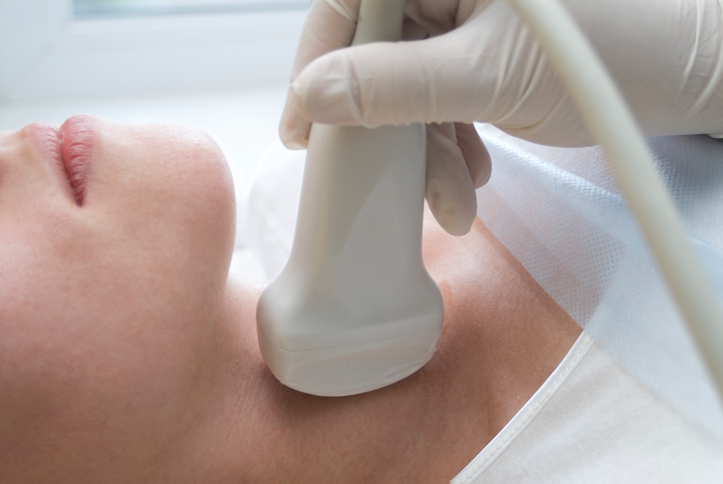
\includegraphics[angle=5,width=0.864\linewidth]{img/ultrasoundNeck.jpg}}
  \cite{TwoViews}
\end{center}
\paragraph{How does it work?}
By using sound waves, there are interactions between the waves and our body.
These waves are weakened to different degrees both on their way in and when reflected back out. This in turn forms an image that doctors can read.

\paragraph{What are the risks?}
The process is harmless and completely free of ionising radiation.

Something to remember is that it can't tell if a tumour is cancerous or not \cite{ACS2020}. 

\section{\faPlusSquare\ X-ray imaging}
Particularly Computer Tomography, known as CT scans, provide important information about tumours and are painless.
\paragraph{How does it work?}
The process is similar to using a flashlight against an object and seeing the shades against a wall.
The opaqueness to x-ray of the area being imaged determines the various shades we see.

Pictures from varying angles are taken and a computer reconstructs those various shades into sectional images, revealing details of our insides.  

\paragraph{What are the risks?}
While it is ionising radiation, the use of CT scans provides life-saving information.
The dosages used in medical imaging are not high enough to establish a risk \cite{ACOG2017}, but you should converse with your doctor and determine whether the benefits outweigh the possible risks, regardless of how small they may be.

Contrasting agents, used to produce better diagnostic information, may also be used.
They are generally safe, but once again, avoided unless absolutely necessary to provide better information. 
 

\section{\faFemale\ Should I be concerned if I'm pregnant?}
Particularly radiography may sound scary, but even if you are pregnant there is little reason for concern \cite{ACOG2017, AmFam1999}.

You should not expect any side effects, but to be safe you may be given a lead vest to protect your belly from the x-ray radiation.
\section{What should I expect from treatment?}


\paragraph{Surgery}
\paragraph{Radiation}
\paragraph{Chemotherapy}
\paragraph{Immunotherapy}.
\clearpage
\clearpage
\bibliography{bibliography}
\end{document}